%%%%%%%%%%%%%%%%%%%%%%%%%%%%%%%%%%%%%%%%%%%%%%%%%%%%%%%%
%%%%%%%%%%%%%%%%%%%%%%%%%%%%%%%%%%%%%%%%%%%%%%%%%%%%%%%%
%  PREAMBLE : USE AT THE BEGINNING OF EVERY PRESENTATION 
%%%%%%%%%%%%%%%%%%%%%%%%%%%%%%%%%%%%%%%%%%%%%%%%%%%%%%%%
%%%%%%%%%%%%%%%%%%%%%%%%%%%%%%%%%%%%%%%%%%%%%%%%%%%%%%%%
\documentclass[11pt]{beamer}

\usepackage{appendixnumberbeamer}

\usepackage{booktabs}
\usepackage[scale=2]{ccicons}

\usepackage{pgfplots}
\usepgfplotslibrary{dateplot}

\usepackage{fontspec}
\defaultfontfeatures{Ligatures=TeX}
\setsansfont{Roboto}[
    Path = /usr/local/texlive/2017/texmf-dist/fonts/truetype/google/roboto/,
    Extension =.ttf,
    ItalicFont = *-RegularItalic,
    BoldFont = *-Black,
    UprightFont = *-Regular ]

% set beamer fonts
\setbeamerfont{title}{size=\huge}
% \setbeamerfont{itemize/enumerate body}{size=\large}
% \setbeamerfont{itemize/enumerate subbody}{size=\normalsize}
% \setbeamerfont{itemize/enumerate subsubbody}{size=\small}
\setbeamerfont{frametitle}{size=\Large}
\DeclareMathSizes{12}{12.5}{9}{9}

% Change default title color
\usepackage{xcolor}
\definecolor{myblue}{RGB}{18, 65, 104}  % title color
\definecolor{myhl}{RGB}{21, 126, 186}   % texthighlight color
\definecolor{myblack}{RGB}{43, 40, 40}
\setbeamercolor{titlelike}{parent=structure,fg=myblue}

% Chaneg bullet points
% \setbeamertemplate{itemize items}{\setlength\itemsep{1em}}
\setbeamercolor*{item}{fg=myblue}

% disable navigation
\setbeamertemplate{navigation symbols}{}

% Add progressbar
\setbeamercolor{progress bar progress}{use=progress bar,bg=progress bar.fg}
\defbeamertemplate{footline}{progress bar}{%
    \ifnum\thepage>1\relax
        \dimen0=\paperwidth%
        \multiply\dimen0 by \insertframenumber
        \divide\dimen0 by \inserttotalframenumber
        \edef\progressbarwidth{\the\dimen0}

        \leavevmode%
        \begin{beamercolorbox}[wd=\paperwidth,ht=2.25ex,dp=1ex]{progress bar}
        \begin{beamercolorbox}[wd=\progressbarwidth,ht=2.25ex,dp=1ex]{progress bar progress}
        \end{beamercolorbox}%
    \end{beamercolorbox}%
\fi
}
\setbeamertemplate{footline}[progress bar]
\setbeamercolor{progress bar}{fg=myblue,bg=white!70!black}


% disable "Figure:" in the captions
\setbeamertemplate{caption}{\tiny\insertcaption}
\setbeamertemplate{caption label separator}{}

% set new command for code/highlight
\newcommand{\code}[1]{\texttt{#1}}
\newcommand{\hl}[1]{\textcolor{myhl}{#1}}

% use package for text positioning
\usepackage[absolute,overlay]{textpos}
%%%%%%%%%%%%%%%%%%%%%%%%%%%%%%%%%%%%%%%%%%%%%%%%%%%%%%%%

%----------------
% BEGIN DOCUMENT
%----------------
\graphicspath{{/images/}}

\title{\textbf{Frictional Ageing from Interfacial Bonding and the Origins of Rate and State Friction}}
\date{Feb 4, 2019}
\author{Prithvi Thakur}
\subtitle{Li et al., 2011}

\begin{document}

\maketitle

\linespread{1.3}

\begin{frame}{\textbf{Key Points}}
    \begin{itemize}
        \item Static friction of rocks grows logarithmically with time (ageing). The mechanism for this strengthening is explored in this paper.
        \item Frictional ageing arises from the formation of interfacial chemical bonds. Plastic creep cannot explain the ageing at the nm scale.
        \item A single contact (asperity) at the nanoscale level is isolated to investigate the physical origins of ageing process.
    \end{itemize}
\end{frame}
\begin{frame}{\textbf{Key Points}}
    \begin{itemize}
        \item Frictional ageing is length-scale dependent: relatively larger at smaller scales.
        \item Logarithmic dependence is attributed to the rate of the chemical reaction slowing with time.
    \end{itemize}
\end{frame}

\begin{frame}{\textbf{Methods}}
    \begin{itemize}
        \item Single Asperity Slide-Hold-Slide friction experiment.
        \item Nanoscopically sharp oxidized silicon tips and oxidized silicon wafers using Atomic Force Microscope.
        \item Second experiment between Silicon and Diamond/Graphite shows very contrasting results: little or no ageing.
    \end{itemize}
\end{frame}

\begin{frame}{\textbf{Discussion}}
    \begin{figure}
        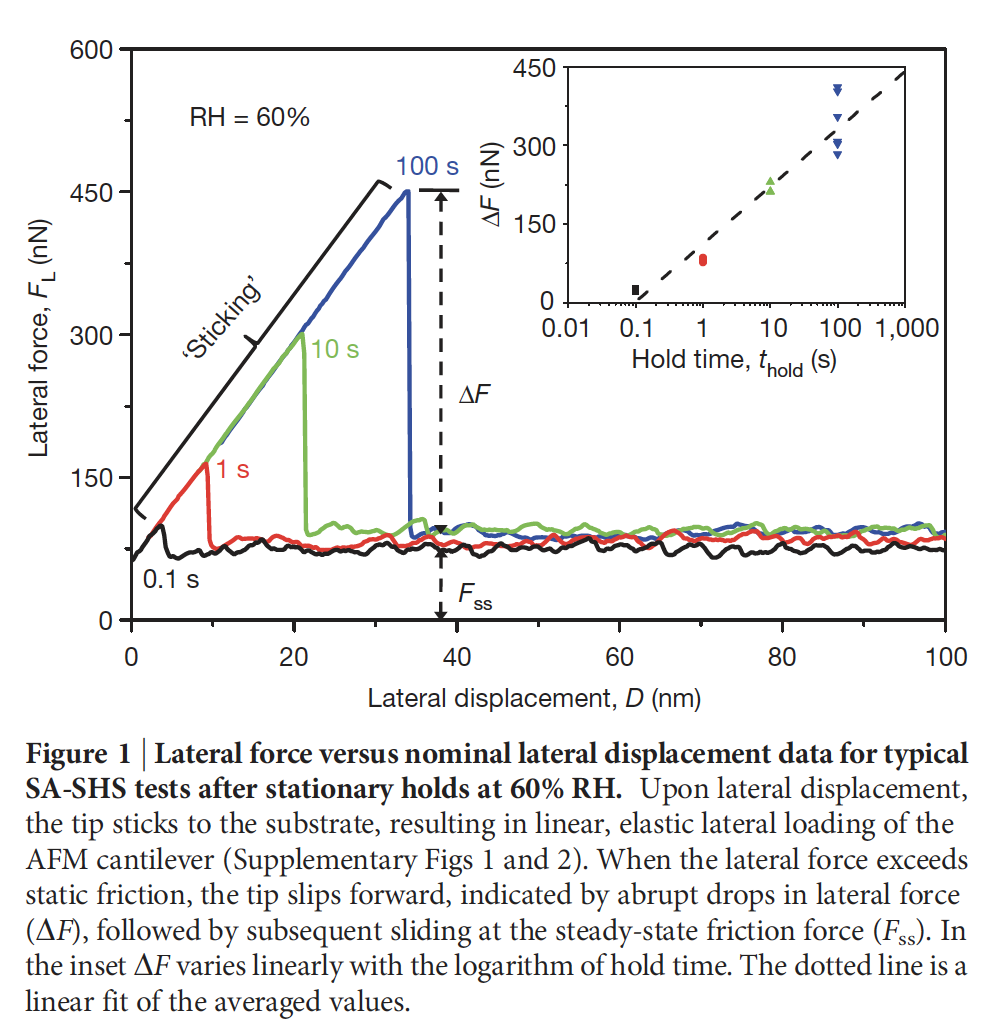
\includegraphics[width=0.6\linewidth]{images/1}
    \end{figure}
\end{frame}
\begin{frame}{\textbf{Discussion}}
    \begin{figure}
        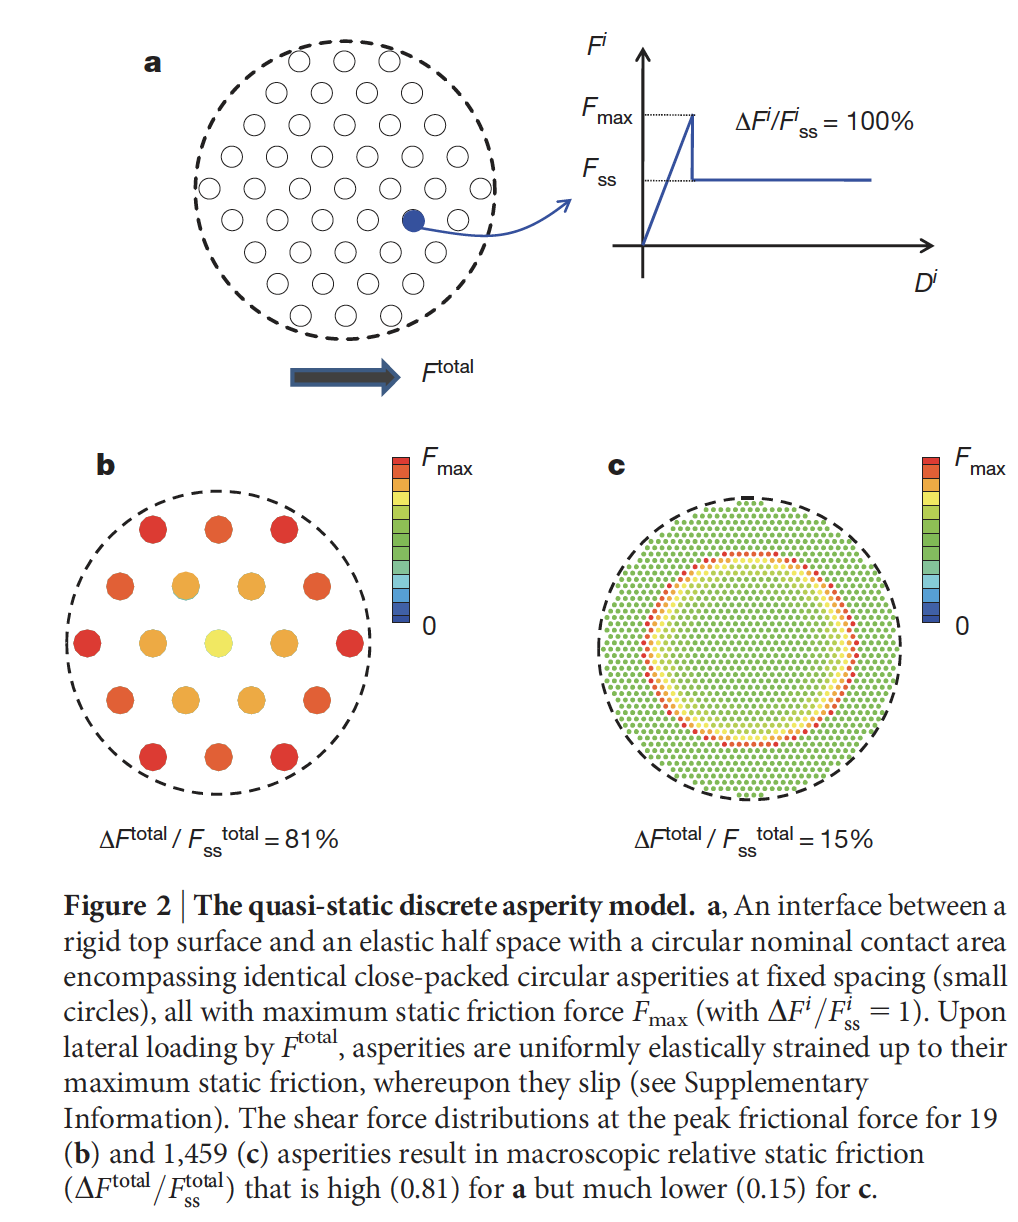
\includegraphics[width=0.6\linewidth]{images/2}
    \end{figure}
\end{frame}
\begin{frame}{\textbf{Discussion}}
    \begin{figure}
        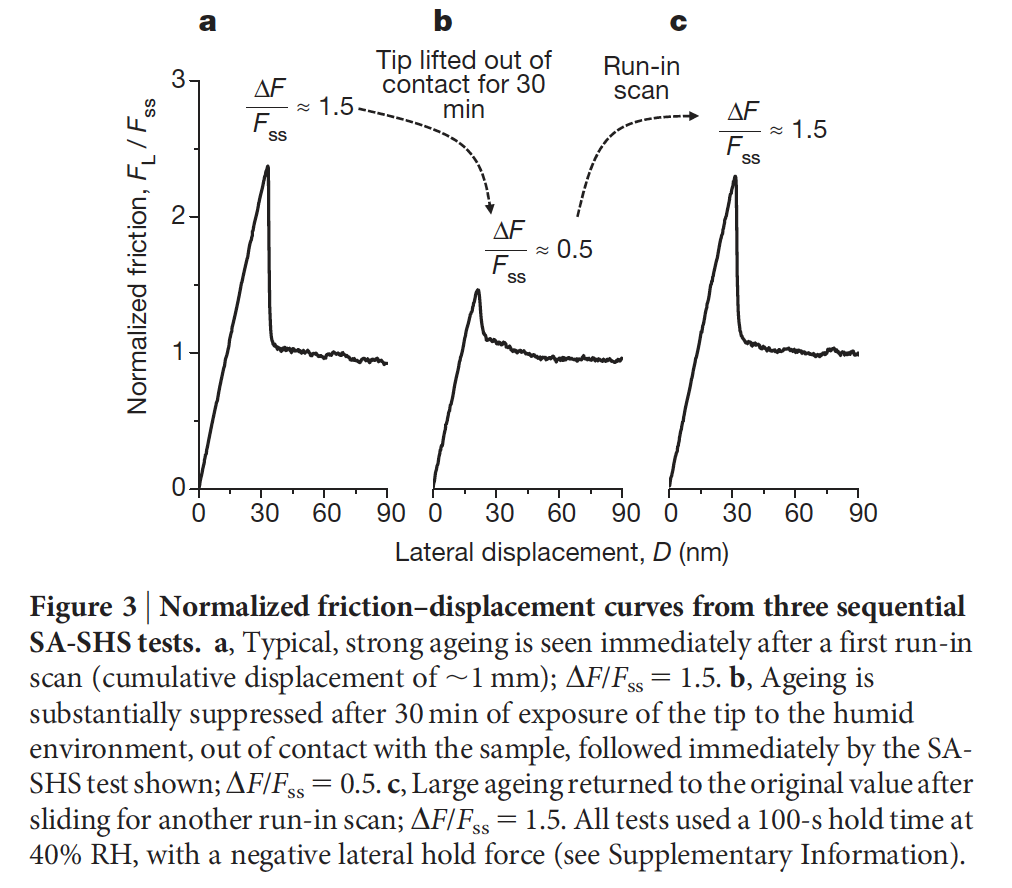
\includegraphics[width=0.6\linewidth]{images/3}
    \end{figure}
\end{frame}
\begin{frame}{\textbf{Discussion}}
    \begin{figure}
        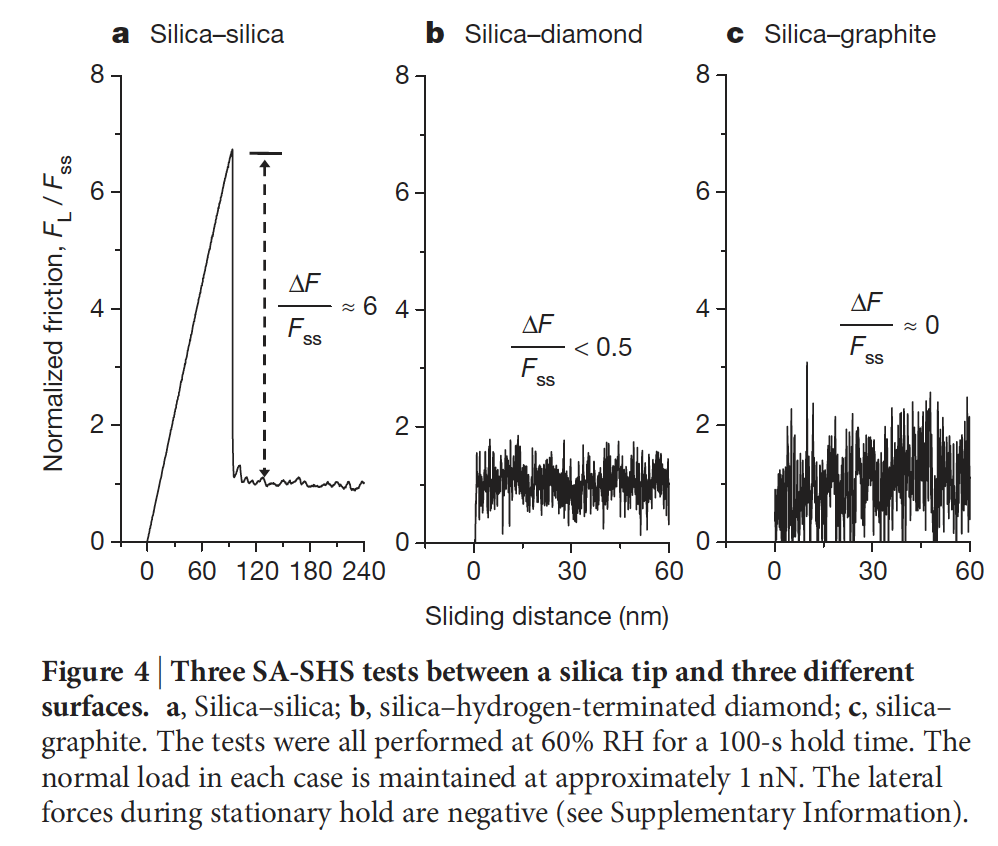
\includegraphics[width=0.6\linewidth]{images/4}
    \end{figure}
\end{frame}

\begin{frame}{\textbf{Questions and Discussions}}
    \begin{itemize}
        \item Larger contacts will have lower macroscopic ageing effect: The difference is attributed to multi-asperity vs single asperity; exposure to water and other contaminants. These mechanisms are still not sufficient to explain two orders of magnitude difference in the ageing. 
        \item Chemical bond formation should imply different rocks would have different friction properties. But they are usually considered constant across the whole earth.
    \end{itemize}
\end{frame}

\end{document}
